\section{Turning}
	\subsection{Setup}
		The other option is for the ship to complete a circular turn to change directions.
		This can be modelled by the diagram below.
		\begin{figure}[ht!]
	\caption{Diagram of what happens when Alice turns.}
	\label{fig:turningAlice}
	\centering
	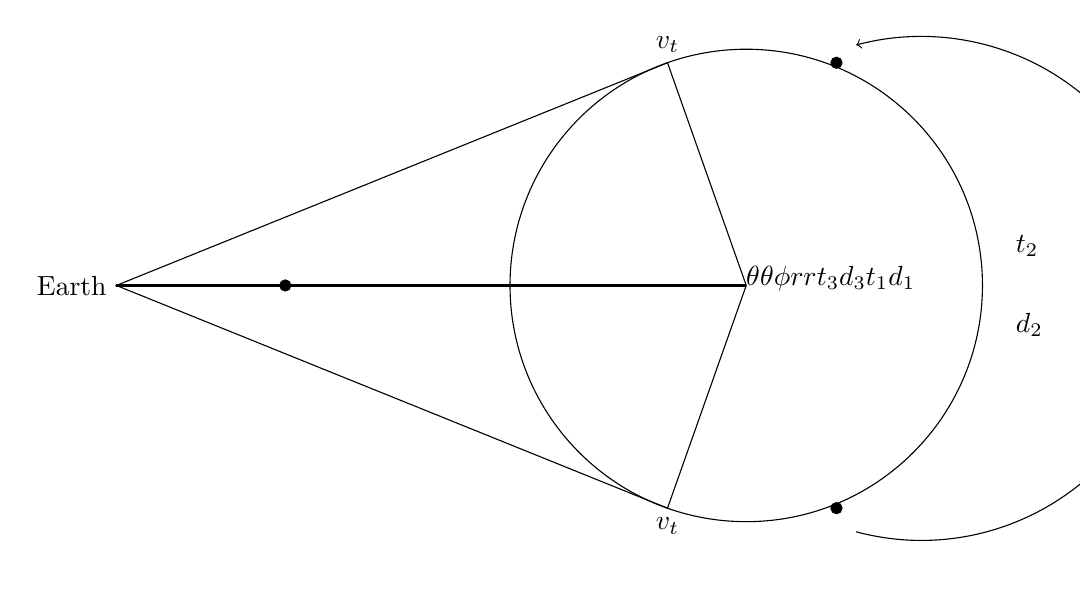
\begin{tikzpicture}
		\coordinate (O) at (0,0);
		\coordinate [label=left:Earth] (E) at (-8,0);
		\coordinate [label=above:$v_t$] (A) at (-1,2.828427125);
		\coordinate [label=below:$v_t$] (B) at (-1,-2.828427125);
		\coordinate [label=right:$\Del t_2$] (T) at (3.3,0.5);
		\coordinate [label=right:$\Del d_2$](D) at (3.3,-0.5);

		\draw (O) circle (3);
		\draw (A) -- (O) -- (B) -- (E) -- cycle;
		\draw[thick](O) -- (E);

		\tkzMarkRightAngle(E,A,O);
		\tkzMarkRightAngle(E,B,O);

		\tkzMarkAngle[size=0.6](A,O,E);
		\tkzLabelAngle(A,O,E){$\theta$};

		\tkzMarkAngle[size=0.6](E,O,B);
		\tkzLabelAngle[pos=-1](E,O,B){$\theta$};

		\tkzMarkAngle[size=0.75](B,O,A);
		\tkzLabelAngle(B,O,A){$\phi$};

		\tkzLabelSegment[above right](O,A){$r$};
		\tkzLabelSegment[below right](O,B){$r$};

		\tkzLabelSegment[above=1.25em](E,A){$\Del t_3$};
		\tkzLabelSegment[above=0.25em](E,A){$\Del d_3$};

		\tkzLabelSegment[below=0.25em](E,B){$\Del t_1$};
		\tkzLabelSegment[below=1.25em](E,B){$\Del d_1$};

		\draw[->] (-0.75,-3.128427125) arc (-105:105:3.2);

		\filldraw[black] (A) circle (2pt);
		\filldraw[black] (B) circle (2pt);
		\filldraw[black] (E) circle (2pt);
	\end{tikzpicture}
\end{figure}

		In this path, the ship will accelerate forward (away from the earth) in a straight line for a time $\Del t_1$.
		The ship will then continue with constant speed around a turn with radius **r** by accelerating towards the centre of the turn.
		The ship will be in this turn for a time $\Del t_2$. Finally, the ship will decelerate as it approaches the  earth for a time $\Del t_3$ until it reaches a halt at its initial position (position of the earth).

		Using this diagram we can set up the following equation: $\Del T_T = \Del t_1 + \Del t_2 + \Del t_3$.

		As shown in the diagram, both $\Del d_1$ and $\Del d_3$ are tangent to the circle which models the turn, and pass through the same point, being the position of the earth.
		As such, we can say that $\Del t_1 = \Del t_3$ and $\Del d_1 = \Del d_3$.

		We then get the following equation: $\Del T_T = 2\Del t_1 + \Del t_2$.

		We must solve for $\Del t_2$ in terms of $\Del t_1$ in order to get a workable equation, so we must set up the following set of 
		equations:
	\subsection{Equations}
		\subsubsection{Known values}
			\begin{description}
				\item[$a$] The acceleration.
				\item[\si{\clight}] The speed of light.
				\item[$T_T$] The total time.
			\end{description}
		\begin{samepagecols}{2}
			\subsubsection{Acceleration distance}
			\begin{align*}
				v &= \si{\clight}\tanh\left(\frac{at}{\si{\clight}}\right)\\
				v_t &= \si{\clight}\tanh\left(\frac{a \Del t_1}{\si{\clight}}\right)\\
				\Del d_1 &= \int \si{\clight}\tanh\left(\frac{a \Del t_1}{\si{\clight}}\right) \dif \Del t_1\\
				\Del d_1 &= \int \frac{\si{\clight}}{a} \times \frac{\sinh\left(\frac{a \Del t_1}{\si{\clight}}\right)}{\cosh\left(\frac{a \Del t_1}{\si{\clight}}\right)} \dif \Del t_1\\
				\Del d_1 &= \frac{\si{\clight}^2}{a} \int \frac{1}{\frac{\sinh\left(\frac{a \Del t_1}{\si{\clight}}\right)}{\cosh\left(\frac{a \Del t_1}{\si{\clight}}\right)}} \dif \Del t_1\\
				\Del d_1 &= \frac{\si{\clight}^2}{a} \ln\left| \cosh\left(\frac{\si{\clight} \Del t_1}{\si{\clight}}\right)\right|\\
				&\frac{a \Del t_1}{\si{\clight}} > 0 \implies \cosh > 0\\
				\Del d_1 &= \frac{\si{\clight}^2}{a} \ln\left(\cosh\left(\frac{\si{\clight} \Del t_1}{\si{\clight}}\right)\right)
			\end{align*}
			\columnbreak
			\subsubsection{Turn distance}
				\begin{align*}
					\tan \theta &= \frac{\Del d_1}{r}\\
					\theta &= \arctan\left(\frac{\Del d_1}{r}\right)
				\end{align*}
				\begin{equation*}
					\phi = 2\pi - 2\theta
				\end{equation*}
				\begin{equation*}
					\Del d_2 = \phi r
				\end{equation*}
			\subsubsection{Turn time}
				\begin{equation*}
					\Del t_2 = \frac{\Del d_2}{v_t}
				\end{equation*}
			\subsubsection{Turn radius}
				\begin{equation*}
					a = \frac{v^2}{r} \qquad r = \frac{v^2}{a}
				\end{equation*}
		\end{samepagecols}
		Using these equations we can substitute into $\Del T_T = 2\Del t_1 + \Del t_2$ to get our final equation in subsection \vref{subsec:disgusting}.
	\subsection{The total time}\label{subsec:disgusting}
		\[\Del t_1 = \Del t_3\]
		\begin{align}
			\Del T_T &= \Del t_1 + \Del t_2 + \Del t_s\nonumber\\
			\Del T_T &= 2\Del t_1 + \Del t_2\nonumber\\
			\Del T_T &= 2\Del t_1 + \frac{\left(2\pi - 2\arctan\left(\frac{\Del d_1}{r}\right)\right) \frac{v^2}{a}}{v}\nonumber\\
			\Del T_T &= 2\Del t_1+\frac{\left(2\pi - 2\arctan\left(\frac{\frac{\si{\clight}^2}{a}\ln\left(\cosh\left(\frac{a\Del t_1}{\si{\clight}}\right)\right)}{\frac{v^2}{a}}\right)\right) v}{a}\nonumber\\
			\Del T_T &= 2\Del t_1+\frac{\left(2\pi-2\arctan\left(\frac{\si{\clight}^2\ln\left(\cosh\left(\frac{a\Del t_1}{\si{\clight}}\right)\right)}{\left(\si{\clight}\tanh\left(\frac{a\Del t_1}{\si{\clight}}\right)\right)^2}\right)\right) \times \si{\clight}\tanh\left(\frac{a\Del t_1}{\si{\clight}}\right)}{a}\nonumber\\
			\Del T_T &= 2\Del t_1+\frac{\left(2\pi-2\arctan\left(\frac{\ln\left(\cosh\left(\frac{a\Del t_1}{\si{\clight}}\right)\right)}{\left(\tanh\left(\frac{a\Del t_1}{\si{\clight}}\right)\right)^2}\right)\right) \times \si{\clight}\tanh\left(\frac{a\Del t_1}{\si{\clight}}\right)}{a}\label{eq:disgusting}
		\end{align}
		This gives us the final equation \eqref{eq:disgusting}.

		It is not possible to isolate for $\Del t_1$ in this equation, so we will have the computer approximate the value and calculate based
		off that.

		For the same reasons stated above, the time dilation over the time frame $\Del t_1$ is equal to the time dilation over the time frame
		$\Del t_3$. Given that the magnitude of velocity over the turn will be equal, we can calculate the time dilation over the time frame
		$\Del t_2$ without summation. Thus, the simulator will only calculate the time dilation initial time step, then multiply by 2, then 
		it will sum the result with the dilation over the time step for the turn.

		The program to solve it was written by David White, and the source code is in appendix \vref{appendix:sourceCode}.

		The simulator will use the above approximations for time dilation in each of the scenarios listed above to approximate the optimal
		condition for each scenario; being the trip time (the time relative to Alice) which yields an arrival within minutes of the
		end of Trump's presidency.

		The simulator will provide the following information:
		\begin{itemize}
			\item The number of seconds between the end of trumps presidency and the arrival of the space ship.
			\item The trip time, the total time that the astronaut spends in the ship (relative to him).
			\item The total time that the astronaut spends in the ship (relative to people on earth).
			\item The total time skipped (the discrepancy between the time the astronaut experiences and the time people on earth experience).
		\end{itemize}
